% -*- root: ../../main.tex -*-
\section{Mediator}
\label{sec:mediator_design}

Dopo un attento studio delle \textbf{specifiche} sviluppate nella fase di analisi è emerso un importante \textbf{problema di interazione} fra alcuni \textbf{componenti cardine}. Come è stato ribadito in TODO il design è stato sviluppato cercando di tenere conto dei principali \textbf{requisiti di qualità} e \textbf{buona progettazione}. Questo grado di \textbf{estendibilità} e \textbf{modularizzazione} si è esplicitato nella definizione di una architettura (\texttt{Core}) \textbf{espandibile a richiesta} verso un modello \textbf{client-server} ad \textbf{attori} (\texttt{Core + Actor}).

Mantenere un \textbf{core unico} e \textbf{polifunzionale} non è semplice ed è necessario ridefinire gli elementi mobili utilizzando il cosidetto \texttt{loose coupling}. 

\subsection{Il Problema}
Nell'architettura core definita in fase di progettazione il problema risiede essenzialmente nella gestione del passaggio da \textbf{single-player} game a \textbf{multiplayer}. 

\paragraph{Single-player:}
Nella versione single-player il sistema di gioco si appoggia sul cosiddetto \texttt{GameEngine} il quale è in grado di \textbf{calcolare autonomamente gli aggiornamenti} da inviare alla/e schermata/e di gioco.

\paragraph{Multiplayer:}
Nel caso multiplayer esiste un \textbf{server unico} a cui sono collegati una serie di \textbf{client}. Il server agisce da leader poiché, possedendo un \texttt{GameEngine} proprio, è in grado di calcolare gli \textbf{aggiornamenti di gioco} a fronte di \textbf{input propri} e \textbf{dei client}. I client, al fine di promuovere \textbf{semplicità}, sono stati concepiti come \textbf{architetture core} private del motore di calcolo \texttt{GameEngine}. Essi in poche parole si presentano come \textbf{attori passivi} che \textbf{acquisiscono aggiornamenti} dal server e li mostrano all'utente attraverso una \textbf{interfaccia grafica}.

Un approccio di questo tipo è molto utile poiché permette di poter utilizzare il server per giocare \textbf{ospitando contemporaneamente la partita in corso}. Inoltre promuove \textbf{leggerezza} e \textbf{riusabilità} dato che i client devono mostrare le \textbf{stesse informazioni} che il server produrrebbe per sé stesso in modalità single-player.

\paragraph{Da Single-player a Multiplayer}
Il problema, come abbiamo detto, si presenta nel passaggio da \textbf{single-player a multiplayer} mode. Nel caso di un passaggio a \textbf{server-mode} il sistema dovrà mantenere il core intatto ma dovrà aver cura di \textbf{inviare gli aggiornamenti} non solo all'\textbf{interfaccia locale} ma anche all'\textbf{attore server} (il quale effettuerà un broadcast ai client). Il passaggio a \textbf{client-mode} è ancora più delicato; in questo caso, infatti, sarà necessario spegnere il modulo \texttt{GameEngine} \textbf{dirottando i flussi di informazione} verso il \textbf{client-actor}.

\subsection{La Soluzione}
Al fine di definire una soluzione valida ci si è appoggiati su un pattern di design di tipo comportamentale, il \textbf{Pattern Mediator}. Il pattern consiste nella definizione di un \textbf{modulo} esterno a tutti gli altri il cui scopo consiste essenzialmente nella \textbf{mediazione e redirizionamento dei flussi} di dati.

Nel nostro caso il mediator ha lo scopo principe di \textbf{mediare le interazioni} fra quattro componenti fondamentali:
\begin{itemize}
	\item{\textbf{Schermata di Gioco:}}
	Deve essere in grado di inviare comandi al \textbf{proprio}  \texttt{GameEngine} (singleplayer) oppure al \texttt{GameEngine} \textbf{del server} (multi-player). 
	\item{\textbf{Engine:}}
	Riceve i comandi dal \texttt{GameScreen} (singleplayer) o \texttt{GameScreen} dei client e li elabora producendo un \textbf{nuovo aggiornamento}. 
	\item{\textbf{Attore Client:}}
	Può essere concepito come un \texttt{Core} munito solo di un unico \texttt{GameScreen}.
	\item{\textbf{Attore Server:}}
	Può essere concepito come un \texttt{Core} agganciato a un numero di \texttt{GameScreen} variabile.
\end{itemize}
Al fine di gestire al meglio le interazioni è stato scelto di implementare un \textbf{approccio basato su eventi} che è stato poi realizzato in \textbf{due versioni molto simili}:
\begin{itemize}
	\item{\textbf{Mediator Observer:}}
	Il \textbf{Mediator} è stato implementato sfruttando il \textbf{pattern observer ad eventi}.
	\item{\textbf{Mediator Handler:}}
	Il \textbf{Mediator} è stato implementato sfruttando il \textbf{pattern ad handler} basato su \textbf{eventi}.
\end{itemize}

Come vediamo in figura \ref{fig:mediatorObserver} la prima scelta porta come vantaggio una \textbf{maggiore strutturazione} e \textbf{rigidità} del pattern.

\begin{figure}[H]
	\centering
	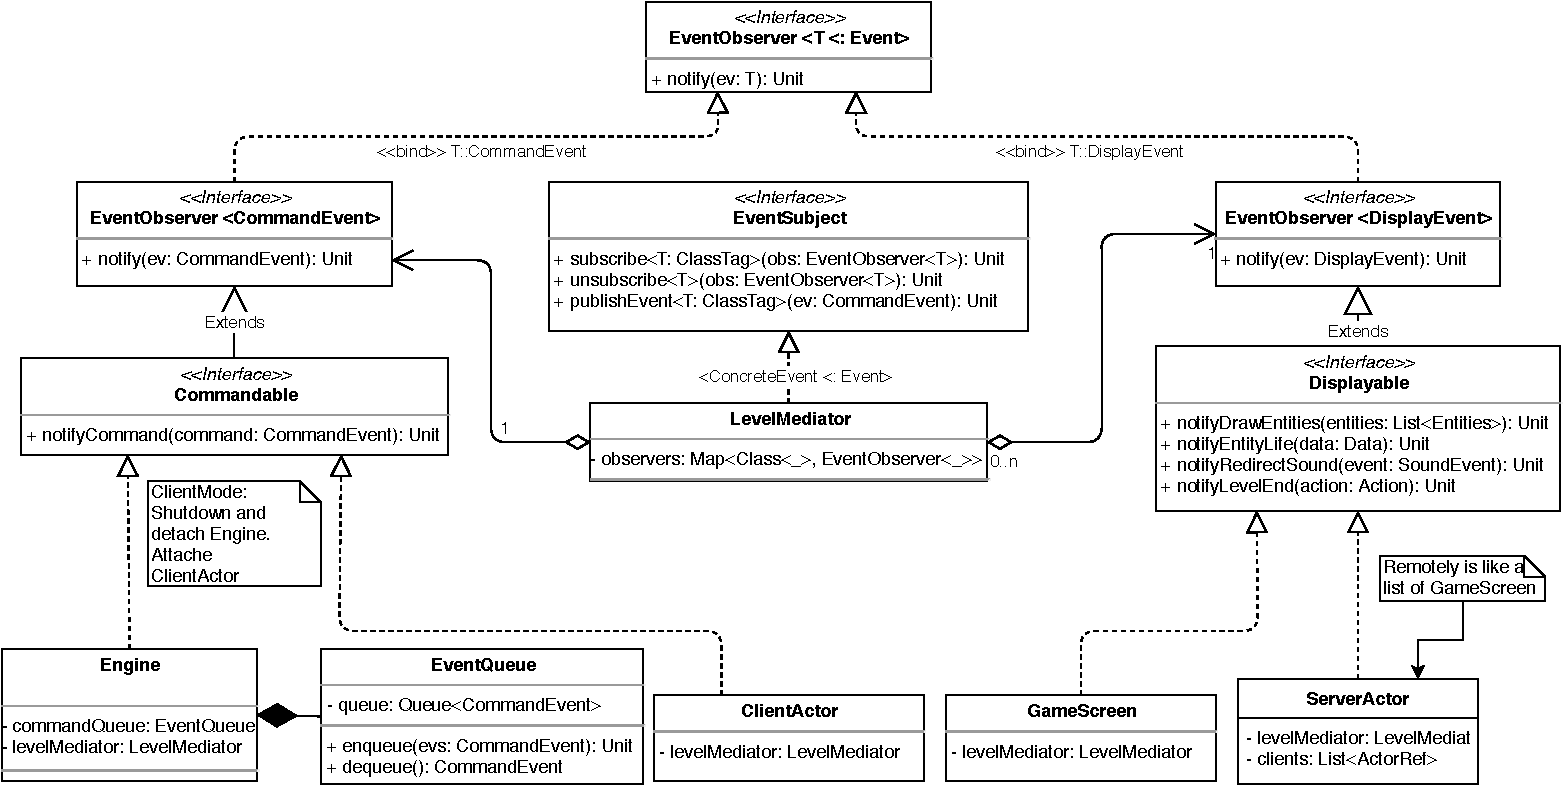
\includegraphics[width=0.99\columnwidth]{drawio/mediator/mediatorObserver.pdf}
	\caption{Design del Mediator basato su observer.}
	\label{fig:mediatorObserver}
\end{figure}

La versione basata su observer è stata poi rivista in un \textbf{approccio} maggiormente \textbf{funzionale} introducendo la struttura ad \textbf{handlers} (fig: \ref{fig:mediatorHandler}).
\begin{figure}[H]
	\centering
	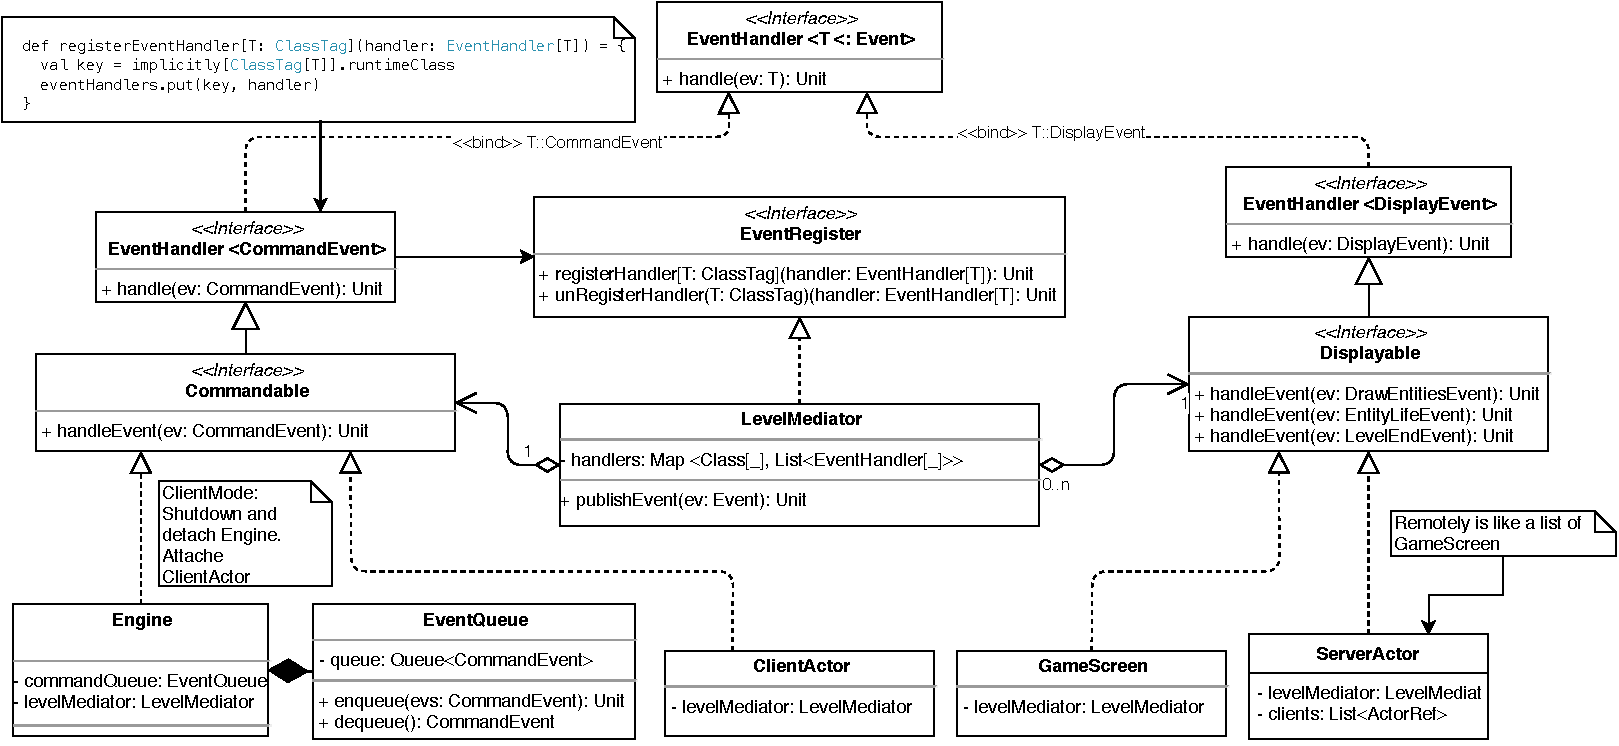
\includegraphics[width=0.99\columnwidth]{drawio/mediator/mediatorHandler.pdf}
	\caption{Design del Mediator basato su handlers.}
	\label{fig:mediatorHandler}
\end{figure}

Utilizzando questo approccio si ha una \textbf{maggiore flessibilità} correlata inoltre da \textbf{performance migliori} poiché ogni handler rappresenta del \textbf{codice associato ad un evento immediatamente eseguibile}.